\section{Modellering}\label{section:Modellering}
I denne sektion vil der blive udarbejdet matematiske modeller for alle dele af systemet. Der vil være tale om et elektronisk system (motor og feedback), der er koblet til et mekanisk system (motorakslen, rammerne og den udveksling, der forbinder dem). 

\subsection{Motor og Pan/Tilt-system}
Motoren består af en elektromagnetisk rotor, og en stator med en permanent magnet. Den permanente magnet sørger for at magnetfeltet, der påvirker rotoren, er nogenlunde konstant - dette forsimpler udledningen af motormomentet $T_{m}$, da det er lineært afhængigt af magnetfeltet og strømmen $i_{a}$ igennem rotorvindingerne se ligning \ref{eq:motormoment}. Motorkonstanten $K_{m}$ er afhængig af permeabiliteten i permanent magnetens materiale og kan bestemmes eksperimentielt \cite{azevedo2013}.

\begin{equation}\label{eq:motormoment}
T_{m}=K_{m}i_{a}(t)
\end{equation}

Den elektriske del af motoren kan modelleres simpelt som en modstand $R_{a}$, der beskriver den samlede modstand i vindingerne, i serie med en spole $L_{a}$, som beskriver motorens induktans. Problemet med denne model er, at den ikke tager højde for den modsatrettede spænding, der genereres i motorvindingerne, når rotoren er i bevægelse. Denne spænding er lineært afhængig af rotorens omdrejningshastighed og kan modelleres som en spændingskilde i serie med modstanden og spolen se figur \ref{fig:motor_sch}. $V_{b}=K_{e}\omega(t)$, hvor $V_{b}$ er den modsatrettede spænding, $K_{e}$ er motorens elektriske konstant og $w(t)$ er omdrejningshastigheden i rad/s.\\



\begin{figure}
	\centering
	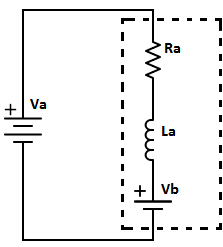
\includegraphics[width=0.3\textwidth]{Billeder/Motormodel.png}
	\caption{Her ses diagrammet af den omtalte motormodel}
	\label{fig:motor_sch}
\end{figure}

Ved hjælp af Kirchoff's lov om spænding kan man nu udlede en differentialligning der relaterer alle elementerne efter spændingen over dem.

\begin{equation}\label{eq:DE_motor_1}
V_{a}=i(t)R_{a}+L_{a}\dfrac{di(t)}{dt}+K_{e}\omega(t)
\end{equation}

Den mekaniske del af motoren kan beskrives som det moment der genereres XXXX *Genereres af hvad?*og driver en belastning. Momentet for enhver roterende masse kan beskrives ved Newton's 2. lov \\
\begin{equation}\label{eq:newtons_2.Lov}
T_{netto}=J\alpha(t)
\end{equation}
hvor $J$ er intertimomentet og $\alpha$ er vinkelaccelerationen. Denne ligning kan bruges til at beskrive nettomomentet for motoren og belastningen. 

\begin{equation}\label{eq:nettomoment}
T_{netto}=T_{m}-T_{f}
\end{equation}

Ligning \ref{eq:motormoment} fortæller noget om momentet fra motoren, men det er også nødvendigt at have en dæmpende effekt i form a friktion med i modellen, for at den kan svare til virkeligheden. Det modsatrettede moment fra friktionen kan approksimeres til at være lineært afhængigt af akslens omdrejningshastighed - denne linearitet kan beskrives ved ligning \eqref{eq:modsatfriktion}
\begin{equation}\label{eq:modsatfriktion}
T_{f}=b\omega(t)
\end{equation}
hvor $b$ er en friktionskonstant.\\Hvis ligning \ref{eq:motormoment},\ref{eq:newtons_2.Lov} og \ref{eq:modsatfriktion} substitueres ind i ligning \ref{eq:nettomoment}, hvor et friktionsmoment trækkes fra motormomentet, dannes en differentialligning, der afhænger af rotorens omdrejningshastighed.

\begin{equation}\label{eq:DE_motor_2}
J\dfrac{d\omega(t)}{dt}=K_{m}i(t)-b\omega(t)
\end{equation}

Ligning \ref{eq:DE_motor_1} og \ref{eq:DE_motor_2} beskriver tilsammen motoren og dens belastning ved at relatere spændingen over motorterminalerne til omdrejningshastigheden. Det er ydermere muligt at beregne en vinkelposition- eller acceleration ved henholdsvis at integrere eller differentiere vinkelhastigheden.


Ved at laplace-transformere ligning \ref{eq:DE_motor_1} og \ref{eq:DE_motor_2} findes overføringsfunktionen $\dfrac{\omega(s)}{V_{a}(s)}$ ved at substituere for $I(s)$. Forholdet findes hvis der antages at startbetingelserne $\omega_{0}$ og $i_{0}$ er lig med nul, og at der ikke er noget \textit{disturbance moment} $T_{d}$.

\begin{equation}
G(s)=\dfrac{\omega(s)}{V_{a}(s)}=\dfrac{K_{m}}{(L_{a}s+R_{a})(Js+b)+K_{m}K_{e}}
\end{equation}

Det er muligt at forsimple systemet ved at se bort fra den elektriske del af motoren's transiente forløb. Det kan lade sig gøre fordi tidskonstanten $\frac{L_{a}}{R_{a}}$ er meget mindre end tidskonstanten for den mekaniske del $\frac{J}{b}$. I s-domænet vil det svare til at polen fra den elektriske del af motoren, befinder sig meget længere til venstre for $j\omega$-aksen end polen fra den mekaniske del. Hvis der ses bort fra den ene af polerne, kan man nu approksimere systemet som et 1.-ordens system, og det er simplere at arbejde med se ligning \ref{eq:Overfoeringsfunktion}.

\begin{equation} \label{eq:Overfoeringsfunktion}
G(s)=\dfrac{\omega(s)}{V_{a}(s)}=\dfrac{K_{m}}{R_{a}(Js+b)+K_{m}K_{e}}
\end{equation}

Der er nu 2 muligheder for at realisere sit system: Der kan laves en \textit{White Box Model}, hvor der, gennem forsøg, findes frem til alle konstanter i motoren og derigennem bestemmer en passende controller. der kan også laves en \textit{Grey Box Model}, hvor der måles step respons for motorens omdrejningshastighed i forhold til spændingen over motorterminalerne. Ud fra denne respons kan der så aflæses en tidskonstant og et dc-gain, og det er alt der behøves for at kunne beskrive et 1.-ordens system. 

\begin{equation}\label{eq:tf_pan_tilt}
G(s)=\dfrac{\omega(s)}{V_{a}(s)}=\dfrac{K}{\tau s+1}
\end{equation}

På figur \ref{fig:time_constant} ses step-respons for et 1.-ordenssystem. Alene ud fra denne graf kan DC-gain'et findes $K$ samt tidskonstanten $\tau$.

\begin{figure}[H]
			\begin{center}
			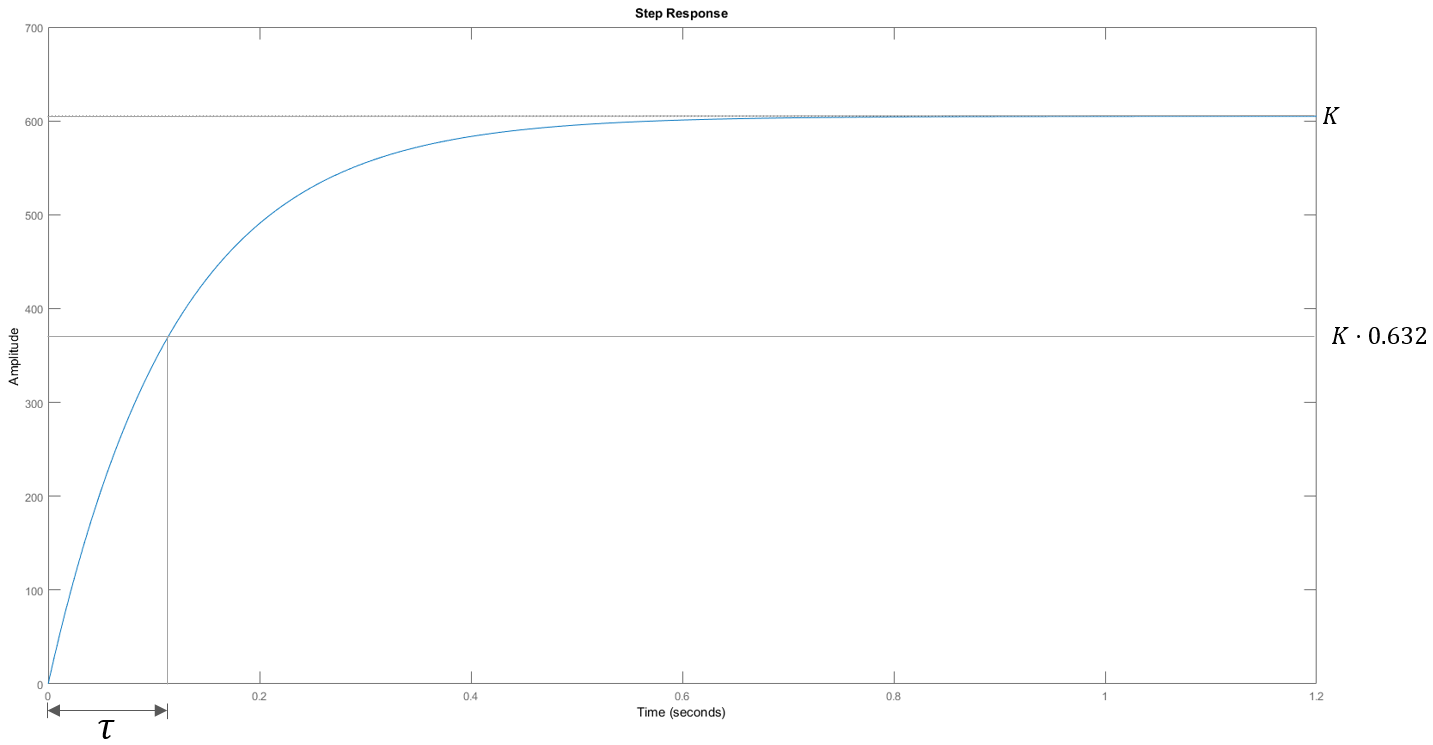
\includegraphics[width=0.9\textwidth]{Billeder/Time_Constant.PNG}
			\end{center}
			\caption{Her ses step-respons for et 1.-ordenssystem, der gør det muligt at aflæse konstanterne $K$ og $\tau$.}
			\label{fig:time_constant}
\end{figure}